\documentclass[twocolumn,fleqn,8pt]{article}  % fleqn left alligns all equations. 
\usepackage[english]{babel} 
\usepackage[latin1]{inputenc} 
\usepackage{times} 			% Default times font style
\usepackage[T1]{fontenc} 	% Font encoding
\usepackage{amsmath} 		% Math package
\usepackage{mathtools} 		% Adds the declare paired 
							% delimeter command to make costom \abs and \norm
\usepackage{breqn}		 	% Adds dmath environment for automated brakeline
\usepackage{xfrac}			% Adds slanted fractions (sfrac)
\usepackage{cancel}			% Adds the cancel command, a slash through the symbol(s)
\usepackage{tabularx}		% Adds adjustable width on tabulars
\usepackage{cuted}			% Adds the \strip command, pagewidth text in a twocolumn
							% environment. 
\usepackage{hyperref}		% Adds the function \url{website}. 
							% Color library. The options allows using names of colors.
\usepackage[usenames,dvipsnames,svgnames]{xcolor}			
\usepackage{geometry}		% Change paper properties such as size. 
\usepackage{fancyhdr}		% Adds customizable headers and footers. 
\usepackage{tikz}
\usepackage{tikz-3dplot}		
\usepackage{blindtext}
\usepackage{titlesec}		% Can change properties of sections, such as color. 
\usepackage{colortbl}
\usepackage[justification=centering]{caption}

% Paper properties. 
\geometry{margin=2cm}
\setlength{\columnsep}{20pt}
\pagestyle{fancy}
\fancyhead[L]{Left }
\fancyhead[R]{Right }

% Assign some new column types. 
\newcolumntype{a}{>{\columncolor{LightCyan}}c}

% Change the definition of \vec to \mathbf
\renewcommand\vec[1]{\mathbf{#1}}
% Start costum \abs \norm 
\DeclarePairedDelimiter\abs{\lvert}{\rvert}%
\DeclarePairedDelimiter\norm{\lVert}{\rVert}%
% Swap the definition of \abs* and \norm*, so that \abs
% and \norm resizes the size of the brackets, and the 
% starred version does not.
\makeatletter
\let\oldabs\abs
\def\abs{\@ifstar{\oldabs}{\oldabs*}}
%
\let\oldnorm\norm
\def\norm{\@ifstar{\oldnorm}{\oldnorm*}}
\makeatother
% End costum \abs \norm 

% Change section formatting. 
\titleformat{\section}
{\color{MediumBlue}\normalfont\Large\bfseries}	% Properties of the title.
{\color{black}\thesection}{1em}{} 			% Properties of the number.
\titleformat{\subsection}
{\color{MediumBlue}\normalfont\large\bfseries}	% Properties of the title.
{\color{black}\thesubsection}{1em}{} 			% Properties of the number.
\titleformat{\subsubsection}
{\color{MediumBlue}\normalfont\large\bfseries}	% Properties of the title.
{\color{black}\thesubsubsection}{1em}{} 			% Properties of the number.

\begin{document}

% Skip the twocolumn environment. This is a hack. The extra "{}" are 
% needed to make the minipage options work. 
\twocolumn[{
	
	\begin{@twocolumnfalse}
	
	\noindent\LARGE{\color{MediumBlue}\textbf
	{Stuff\\}}

	\vspace{-0.1cm}
	\noindent
	\large{\textbf{Daniel Marelius Bj\o rnstad$^1$*\\}}
	
	\vspace{-0.1cm}
	
	{\small $^1$Department of Physics, University in Oslo, Norway}\\
	
	\begin{minipage}[t]{0.25\textwidth}
		\small{
		\noindent 
		{\bf Delivered:} Date\\
		
		{\bf*Correspondance:} \\
		Email (D.M.B.)}
	\end{minipage}
	\vspace{0.7cm}
	\begin{minipage}[t]{0.75\textwidth}
		% The hack resets fontsize it seems. 
		\fontsize{10pt}{12pt}\selectfont
		
	\end{minipage}
	
	\end{@twocolumnfalse}
	
}]
\clearpage

\section{Implementation}
\subsection{Implementation in C++}
\subsubsection{VMCSolver.cpp}
Simulations run on c++ objects called VMCSolver. There are 3 VMCSolvers
implemented in the code.\\
"VMCSolver" - Contains the simulation environment for the hydrogen-like wave
function simulator.\\
"VMCSolverGto" - Contains the simulation environment for the GTOs, can only run
without importance sampling.\\
"VMCSolverGtoI" -Contains the simulation environment for the GTOs, can only run
with importance sampling.\\

The reason for splitting the solvers was that code gradually became too complex
to run in the same object. All solvers has a method which is called
runSingleParticleStep. This method is not run by the solver but must be called
by the user for every particle and for every cycle in the simulation. 
This makes the simulation run directly in the code of the user and not 
as an run simulation method in the in the object. The runSingleParticleStep method
takes the particle number $i$ as an parameter. This is the main difference between
this program and conventional simulatiors. 

This difference has the following major effects: 
{\color{MediumBlue}\bf1.} The user is responsible to run the code with the
correct particle $i$ over the total number of particles. If not, the code will
do an array out of bounds segmentation fault or do a wrong integration.
 {\color{MediumBlue}\bf2.} The user
can easily change the simulation while running, if desired. 
{\color{MediumBlue}\bf3.}
All state variables of the solver are current and not saved in any way. This moves
all helper functions outside of the solver object.
Helper functions such as gathering energies in vectors or matrices, 
or doing position histograms. This is a major change that makes seperating the solver
with the extraction of data very easy. 

\subsubsection{Parallelization}
Parallelization was done by simply increasing the number of trials. For every program
that was run, the program would split into 4 threads and run 1 solver each in parallel.

Further parallelization of parts of the code could be possible, but 
would be unessecary because a high number of trials gives better data
(further discussion can be found under Trials vs. BlockSize). 

\subsubsection{Parameter Optimization}
Paramter optimization can be done using different methods, such as conjugate gradient, 
steepest cecent, newtons method, bisection methods or other. For all these methods
it is important to have a good evaluation function of the value and the gradient of the
scalar function, $E_0(\alpha,\beta)$. In the program we implemented an conjugate gradient
method using python and an evaluation function with c++. 

Parameter optimization was done using 1e6 cycles for Helium , 
1e5 cycles for Beryllium and 1e4 cycles for Neon, all with 4 trials. More on this
subject can be found under the Problems Encountered section and the Improvements section.

\subsubsection{Blocking}
Applying blocking on a vector of sample energies can easily be done by simply making
one mean value of a range of samples equal to the block size. 

Though, second to the data integration, making the complete blocking plot was the 
most CPU intensive operation in the program.
Blocking was done in an easy way to get all possible divisions of the full sample length
into blocks via a brute force method\footnote{\url{https://github.com/lastis/FYS4411/blob/master/Project2/src/cpp/vmcsolver/util.h}}.

\subsubsection{Imrovements}
The implementation had some flaws, of the biggest were implementing GTOs and optimizing the
code. 

{\bf GTOs:} GTOs seemed to give correct ground state energies, $E_0$, at high number of cycles
(above 1e5 for Beryllium and Neon). The problem with GTOs, is that they 
{\color{MediumBlue}\bf1.} require a large amount
of CPU time, 10x the one of the hydrogen-like wave function. {\color{MediumBlue}\bf2.}
They are also hard to varify as the simulation is quite robust to human error. If 
the implementation of them are missing a factor or the calculation is somehow not
correct, the code will often run fine and still give an $E_0$ which can seem reasonable. 

The reason for stating GTOs as a problem, was because they did not give the
density plots we expected from Beryllium and Neon.

{\bf Optimization:}
The speed of the code can be improved. This was not a big focus of the project, but
it is very useful for getting results in a timely fashion. The biggest way this
can be improved is by using an external analyzation tool for c++ code. 

A consequence of slow runtime was the convergence of 
the conjugate gradient method for Beryllium and Neon. 
Our parameters were 1e5 cycles for Beryllium and 1e4 cycles for Neon, with 4 trials
on both. We think both of these variables should be at least 10x higher to give
stable $\alpha$, $\beta$ values with more than 2 significant numbers.


\subsection{Problems Encountered}
\subsubsection{Thermalization}
\begin{figure}
	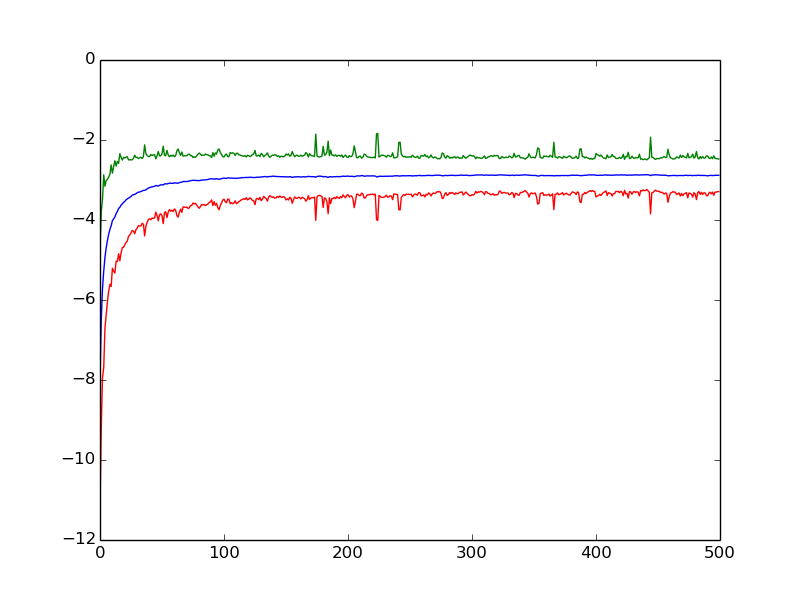
\includegraphics[width=\columnwidth]{../res/plot/helium_04/helium_04.png}
	\caption[caption]{$E_0$ vs. cycle number. 
	 	Trials: 4000. $\alpha = 1.79$. 
	$\beta = 0.4125$}
	\label{fig:helium_04}
\end{figure}
A problem that was encountred for all simulations was that the first samples of every 
trial were not valid samples for the ground state. This problem is not a problem for
Helium as the walkers quickly converges to a stage where they give correct
estimations of the ground state energy
as can be seen in figure (\ref{fig:helium_04}). 

\begin{figure}
	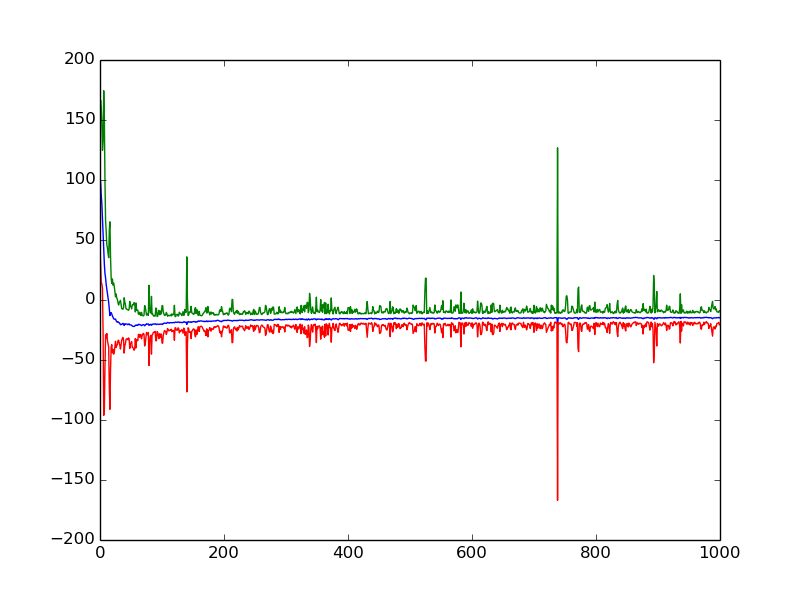
\includegraphics[width=\columnwidth]{../res/plot/beryllium_04/beryllium_04.png}
	\caption{Trials: 4000}
	\label{fig:beryllium_04}
\end{figure}
When increasing particle number and/or using GTOs this becomes an increasing problem
in addition with the increasing in CPU time used for every cycle. In the 
simulations of Beryllium and Neon the rate of which the samples begin to give
valid number for the ground state was increased to about 500 cycles. At 
Figure (\ref{fig:beryllium_04}) show the slow increase in the energy over cycle number. 

\subsubsection{Trial by Trial Variation}
In addition to what we called thermalization, there is the additional problem of getting 
enough sample points to calculate the variance. Increasing the number of trials is often
the main factor to get a function to be smooth over the parameter space. This is thus 
important when using a minimization algorithm, such as Conjugate Gradient, steepest descent
or other methods. If too few trials are run with an optimization method, the 
algorithm will be misguided by the variable results.

\subsubsection{Trials vs. Blocks Size, $n_b$}
A large variability was found when calculating $E_0$ for Beryllium and Neon when 
varying the number of cycles and the number of trials. One would expect
when doing the thermalization anlysis that by skipping a number of cycles in
an order of about 500 should be sufficient to start sampling good values for $E_0$. 
However this is not the case as increasing $n_b > \:$ 1e5 must be used to find
values that look similar to the exact values of $E_0$. 
For hydrogen like wave function the results were found to be:
\begin{align*}
	E_0 = -14.3795 && \alpha = 3.919 && \beta = 0.110 && n_b = \text{1e5}&&\text{Trials} = 4\\
	E_0 = -13.0830 && \alpha = 3.919 && \beta = 0.090 && n_b = \text{1e4}&&\text{Trials} = 4\\
	E_0 = -13.0559 && \alpha = 3.919 && \beta = 0.100 && n_b = \text{1e4}&&\text{Trials} = 160
\end{align*}
These findings suggests that even if the thermalization looks like it
reaches at a platoue at around 500 cycles, this is probably not the case and may continue
to increase to at least 1e4. This applied to all simulations except helium. 


\clearpage

\section{Results}
\subsection{Helium}
\subsubsection{Optimal Parameters}
\begin{figure}
	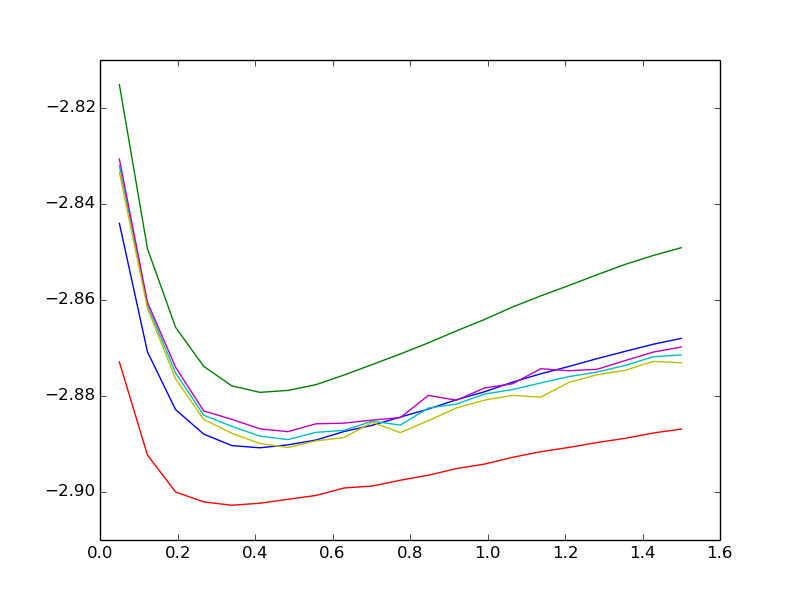
\includegraphics[width=\columnwidth]{../res/plot/helium_01/helium_01.png}
	\caption{Helium hydrogenlike wave function, 1 standard deviation. 
	Points = 20. Trials = 80.	$n_b = \:$1e5. $\alpha = 1.79$}
	\label{fig:helium_01}
\end{figure}
\begin{center}
	\begin{tabular}{| l a c a c |}
	\hline
		& Exact & $E_0$ & $\alpha$ & $\beta$\\
		w Imp. Sampl.& -2.90324 &  -2.89079& 1.79 & 0.4125 \\
		w/o Imp. Sampl. & -2.90324& -2.88864& 1.79 & 0.486 \\
		GTO 3-21G& -2.90324& & - & 0.9925\\
	\hline
	\end{tabular}
\end{center}
{\bf Importance Sampling:}

Importance sampling gave a lower estimation of the ground energy than
the simulation without it. Figure (\ref{fig:helium_01}) shows the difference between
running with and without importance sampling by varying the $\beta$ value. 
$\alpha$ is held constant at 1.79. 
The alpha was chosen to give the lowest energy of the simulation with 
importance sampling and the reason for doing this is that the evaluation of $E_0$ using
importance sampling is considered more correct.
The optimal values for Helium was found the be 
the similar for both importance sampling and with out, but not the same. 

From this point on all simulations will be done with importance sampling. \\

\noindent{\bf GTO Basis 3-21G :}

\begin{figure}
	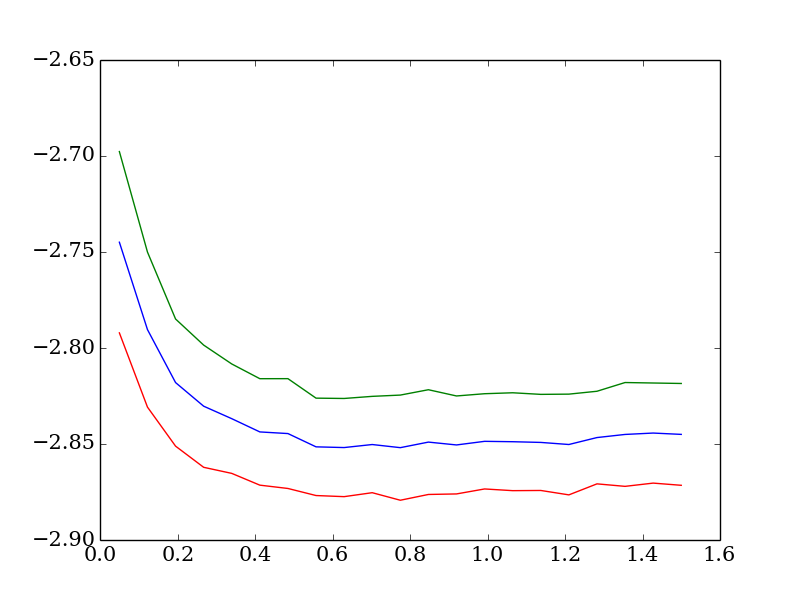
\includegraphics[width=\columnwidth]{../res/plot/helium_05/helium_05.png}
	\caption{Helium GTO importance sampling 1 standard deviation. 
	Points = 20. Trials = 40.	$n_b = \:$1e5.}
	\label{fig:helium_05}
\end{figure}
Figure (\ref{fig:helium_05}) shows the energy as a function of $\beta$. 
The lowest energy is $E_0 = 2.8519$. 
The variance is
roughly the same as with importance sampling
but $E_0$ has not decresead as one would expect. Because lower energies was
not discovered, even with more cycles, the implementation of the GTOs must be seen as flawed.

\subsubsection*{Charge Density}
\noindent{\bf Jastrow Factor:}

The Jastrow factor, which is a function of $\beta$, decides the interaction between
the electrons. Without this factor the electrons does not "see" the other electrons
in the system. This makes the electrons repulse each other and the charge density
is then push out from the nucleus as can be seen in figure(\ref{fig:helium_03}).
\begin{figure}
	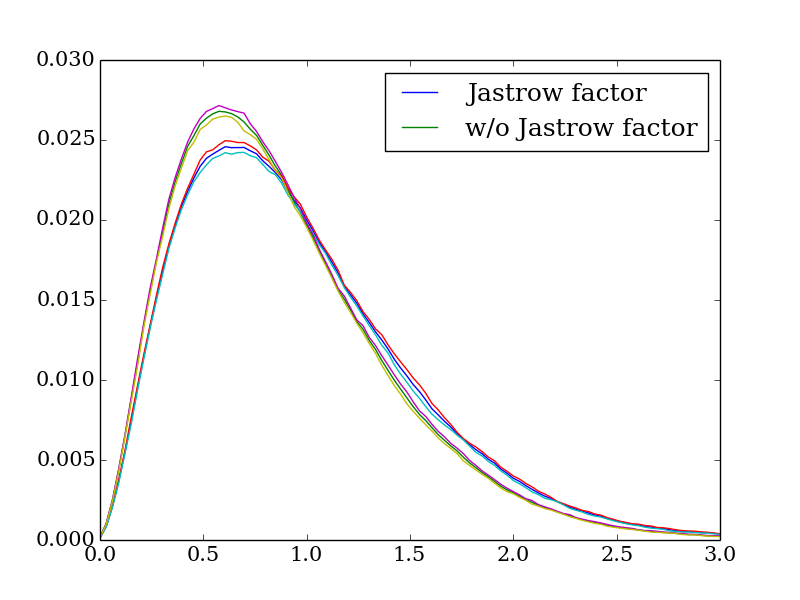
\includegraphics[width=\columnwidth]{../res/plot/helium_03/helium_03.png}
	\caption{Helium hydrogen like wave function, 1 standard deviation. 
	Points = 20. Trials = 40.	$n_b = \:$1e5.}
	\label{fig:helium_03}
\end{figure}

\subsection{Beryllium}
\subsubsection{Optimal Parameters}
\begin{center}
\begin{tabular}{| l a c a c |}
	\hline
		& Exact & $E_0$ & $\alpha$ & $\beta$\\
		Hydrogen like & -14.6664(3 &  -14.3795& 3.9190 & 0.1101 \\
		GTO 3-21G& -14.6664(3)& & - & 0.9925\\
	\hline
\end{tabular}	
\end{center}

\noindent 

The GTO gave a very similar energy of $E_0 = -14.3574$, but requires longer runtimes to give 
stable results. Our suggested runtime variables are at least $n_b > \:$1e5 Trials $>$ 10.
\begin{figure}
	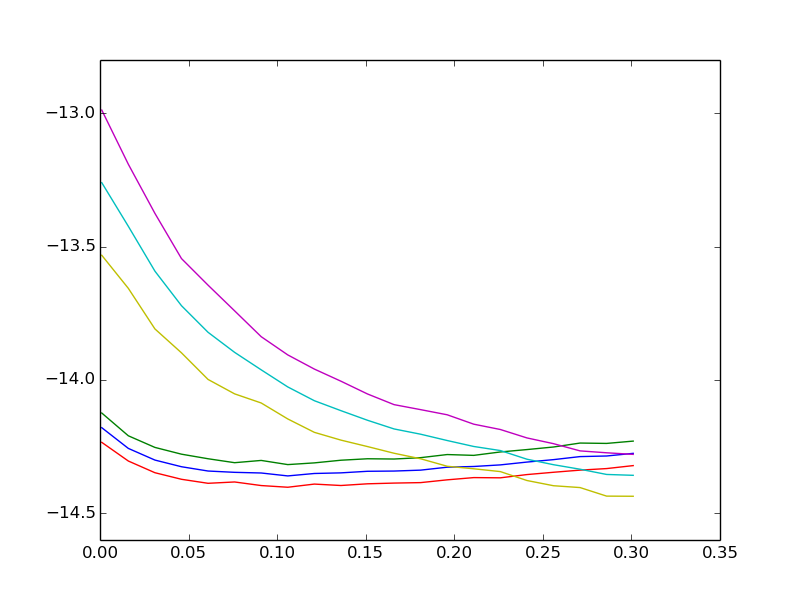
\includegraphics[width=\columnwidth]{../res/plot/beryllium_01/beryllium_01.png}
	\caption{Beryllium, 1 standard deviation. 
	Points = 20. Trials = 4.	$n_b = \:$1e5.}
	\label{fig:beryllium_01}
\end{figure}

\subsubsection{Charge Density}
Using hydrogen like wave functions, the charge density shape coincide with extern 
sources\footnote{\url{http://2012books.lardbucket.org/books/principles-of-general-chemistry-v1.0/section_10/4858a5e15319821597514881b601833b.jpg}} as can be seen in figure
(\ref{fig:beryllium_03}). The addition of the Jastrow factor again makes the
density function more pushed out. 

Using GTOs the density does not look as expected, but rather
looks more like a one with only a single shell, figure(??). This gives further suggestion that 
the implementation of GTO is flawed. An alternative explanation is that using
GTOs does not give correct densities, but rather only correct ground state energy, $E_0$.

\begin{figure}
	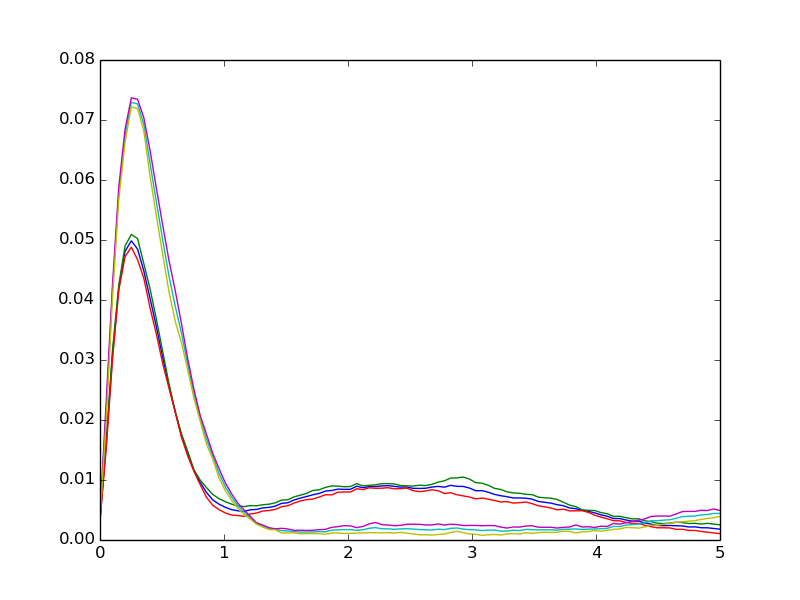
\includegraphics[width=\columnwidth]{../res/plot/beryllium_03/beryllium_03.png}
	\caption{Beryllium, 1 standard deviation. 
	Points = 20. Trials = 4.	$n_b = \:$1e5.}
	\label{fig:beyllium_03}
\end{figure}

\subsection{Neon}
\subsubsection{Optimal Paramters}












\end{document}